\documentclass[border=5pt]{standalone}
\usepackage{tikz}
\usetikzlibrary{arrows.meta, positioning, decorations.pathreplacing, calc}
\usepackage{xcolor}

\definecolor{Garnet}{HTML}{73000A}
\definecolor{NinetyBlack}{HTML}{363636}
\definecolor{SeventyBlack}{HTML}{5C5C5C}
\definecolor{FiftyBlack}{HTML}{A2A2A2}
\definecolor{ThirtyBlack}{HTML}{C7C7C7}
\definecolor{TenBlack}{HTML}{ECECEC}
\definecolor{Atlantic}{HTML}{466A9F}
\definecolor{Congaree}{HTML}{1F414D}
\definecolor{Sandstorm}{HTML}{FFF2E3}

\tikzset{every node/.append style={rounded corners=0pt}}

\begin{document}
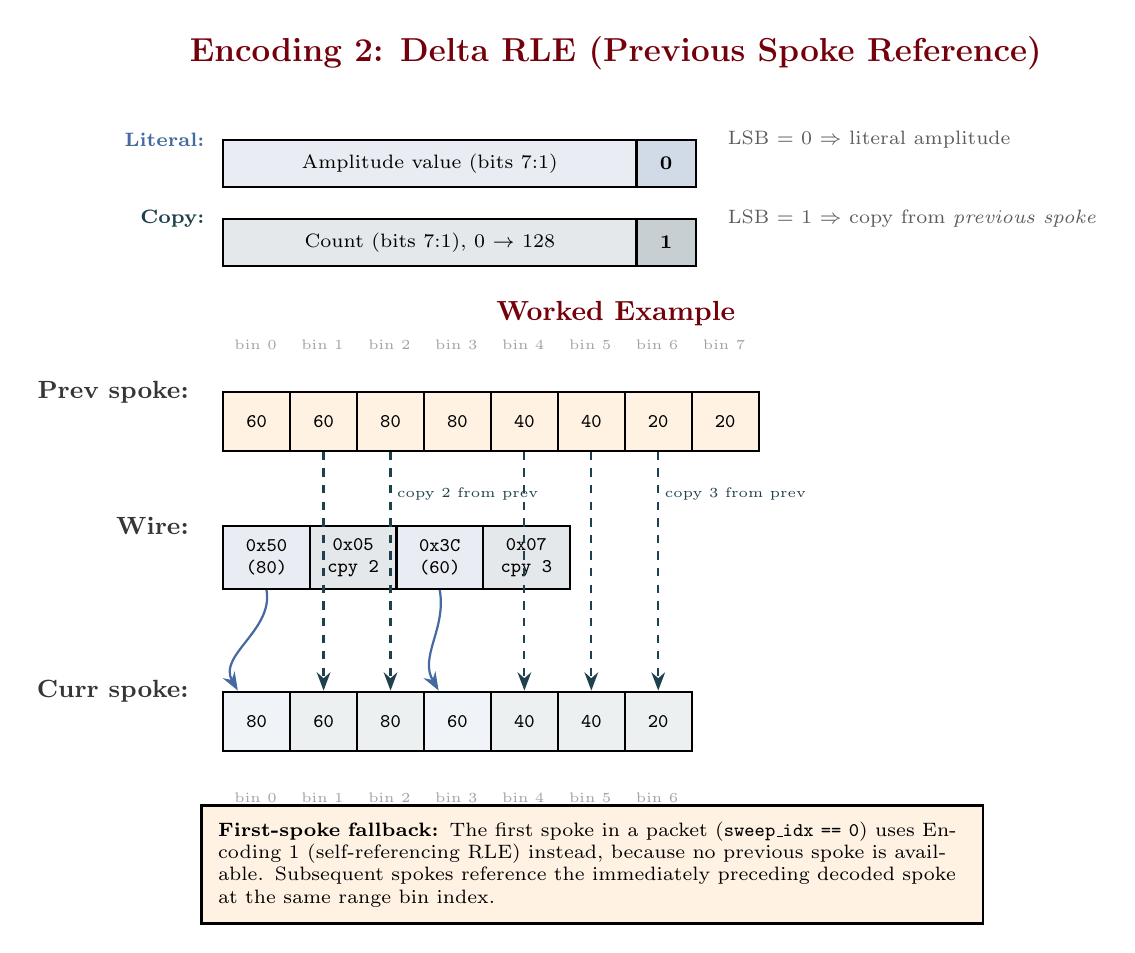
\begin{tikzpicture}[
    cell/.style={draw, thick, minimum width=1.1cm, minimum height=0.8cm, anchor=west, font=\ttfamily\scriptsize, align=center},
    scell/.style={draw, thick, minimum width=0.85cm, minimum height=0.75cm, anchor=west, font=\ttfamily\scriptsize, align=center},
    lbl/.style={font=\small\bfseries, color=NinetyBlack},
    annot/.style={font=\scriptsize, color=SeventyBlack},
]

\node[font=\bfseries\large, color=Garnet] at (5.0, 5.5) {Encoding 2: Delta RLE (Previous Spoke Reference)};

% ── Bit layout ──
\node[font=\scriptsize\bfseries, color=Atlantic, anchor=east] at (-0.1, 4.4) {Literal:};
\node[draw, thick, fill=Atlantic!12, minimum width=5.25cm, minimum height=0.6cm, anchor=west, font=\scriptsize] at (0, 4.1) {Amplitude value (bits 7:1)};
\node[draw, thick, fill=Atlantic!25, minimum width=0.75cm, minimum height=0.6cm, anchor=west, font=\scriptsize\bfseries] at (5.25, 4.1) {0};
\node[annot, anchor=west] at (6.3, 4.4) {LSB = 0 $\Rightarrow$ literal amplitude};

\node[font=\scriptsize\bfseries, color=Congaree, anchor=east] at (-0.1, 3.4) {Copy:};
\node[draw, thick, fill=Congaree!12, minimum width=5.25cm, minimum height=0.6cm, anchor=west, font=\scriptsize] at (0, 3.1) {Count (bits 7:1), 0 $\rightarrow$ 128};
\node[draw, thick, fill=Congaree!25, minimum width=0.75cm, minimum height=0.6cm, anchor=west, font=\scriptsize\bfseries] at (5.25, 3.1) {1};
\node[annot, anchor=west] at (6.3, 3.4) {LSB = 1 $\Rightarrow$ copy from \textit{previous spoke}};

% ── Worked Example ──
\node[font=\bfseries, color=Garnet] at (5.0, 2.2) {Worked Example};

% Previous spoke (top)
\node[lbl, anchor=east] at (-0.3, 1.2) {Prev spoke:};
\node[scell, fill=Sandstorm] (p0) at (0, 0.83) {60};
\node[scell, fill=Sandstorm] (p1) at (0.85, 0.83) {60};
\node[scell, fill=Sandstorm] (p2) at (1.7, 0.83) {80};
\node[scell, fill=Sandstorm] (p3) at (2.55, 0.83) {80};
\node[scell, fill=Sandstorm] (p4) at (3.4, 0.83) {40};
\node[scell, fill=Sandstorm] (p5) at (4.25, 0.83) {40};
\node[scell, fill=Sandstorm] (p6) at (5.1, 0.83) {20};
\node[scell, fill=Sandstorm] (p7) at (5.95, 0.83) {20};

% Bin indices
\foreach \i in {0,...,7} {
    \node[font=\tiny, color=FiftyBlack, above=1pt] at (0.425 + \i*0.85, 1.58) {bin \i};
}

% Wire bytes (left side)
\node[lbl, anchor=east] at (-0.3, -0.5) {Wire:};
\node[cell, fill=Atlantic!12] (w0) at (0, -0.9) {\texttt{0x50}\\(80)};
\node[cell, fill=Congaree!12] (w1) at (1.1, -0.9) {\texttt{0x05}\\cpy 2};
\node[cell, fill=Atlantic!12] (w2) at (2.2, -0.9) {\texttt{0x3C}\\(60)};
\node[cell, fill=Congaree!12] (w3) at (3.3, -0.9) {\texttt{0x07}\\cpy 3};

% Current spoke (bottom)
\node[lbl, anchor=east] at (-0.3, -2.6) {Curr spoke:};
\node[scell, fill=Atlantic!8] (c0) at (0, -2.98) {80};
\node[scell, fill=Congaree!8] (c1) at (0.85, -2.98) {60};
\node[scell, fill=Congaree!8] (c2) at (1.7, -2.98) {80};
\node[scell, fill=Atlantic!8] (c3) at (2.55, -2.98) {60};
\node[scell, fill=Congaree!8] (c4) at (3.4, -2.98) {40};
\node[scell, fill=Congaree!8] (c5) at (4.25, -2.98) {40};
\node[scell, fill=Congaree!8] (c6) at (5.1, -2.98) {20};

% Bin indices below
\foreach \i in {0,...,6} {
    \node[font=\tiny, color=FiftyBlack, below=1pt] at (0.425 + \i*0.85, -3.73) {bin \i};
}

% Vertical arrows: copy from previous spoke
\draw[-{Stealth}, thick, Congaree, dashed] ($(p1.south)$) -- ($(c1.north)$);
\draw[-{Stealth}, thick, Congaree, dashed] ($(p2.south)$) -- ($(c2.north)$);
\node[font=\tiny, color=Congaree, anchor=west] at (2.1, -0.1) {copy 2 from prev};

\draw[-{Stealth}, thick, Congaree, dashed] ($(p4.south)$) -- ($(c4.north)$);
\draw[-{Stealth}, thick, Congaree, dashed] ($(p5.south)$) -- ($(c5.north)$);
\draw[-{Stealth}, thick, Congaree, dashed] ($(p6.south)$) -- ($(c6.north)$);
\node[font=\tiny, color=Congaree, anchor=west] at (5.5, -0.1) {copy 3 from prev};

% Wire to spoke arrows
\draw[-{Stealth}, thick, Atlantic] ($(w0.south)$) to[out=-80, in=120] ($(c0.north west) + (0.2, 0)$);
\draw[-{Stealth}, thick, Atlantic] ($(w2.south)$) to[out=-80, in=120] ($(c3.north west) + (0.2, 0)$);

% Fallback note
\node[draw, thick, fill=Sandstorm, text width=9.5cm, align=left, font=\scriptsize, inner sep=6pt] at (4.7, -4.8)
    {\textbf{First-spoke fallback:} The first spoke in a packet (\texttt{sweep\_idx == 0}) uses Encoding~1 (self-referencing RLE) instead, because no previous spoke is available. Subsequent spokes reference the immediately preceding decoded spoke at the same range bin index.};

\end{tikzpicture}
\end{document}
